\subsection{Hyperparameters can be disentangled and understood}
\label{sec:reason-hps}












Training a deep learning system involves many numerical knobs, termed ``hyperparameters.'' These include optimization hyperparameters such as the learning rate, batch size, momentum, and initialization variance, as well as architecture hyperparameters such as width, and depth.
The large number of hyperparameters in deep learning presents a challenge not only for practitioners, who must tune them carefully in order to achieve optimal performance, but also for researchers, who must grapple with many confounding factors when trying to interpret the outcome of scientific experiments.
It is only in the last few years that the theory community has come to realize that hyperparameters can be disentangled and understood, and that the resulting mathematics is often both useful for practitioners and clarifying for theorists.

This study of hyperparameters bears similarities to the study of the constant parameters governing the behavior of a physical dynamical system.
For example, in a fluid flowing through a pipe, a dimensionless number called the \textit{Reynolds number} computed from the pipe diameter and the fluid's speed, density, and viscosity determines whether flow is laminar or turbulent.
While \textit{solving} for the trajectory of the turbulent fluid is extremely difficult, it is nonetheless very helpful to be able to quickly predict whether flow will be turbulent at all --- and how things change if you scale up the pipe diameter or increase the fluid flow.
Similarly, while solving the optimization dynamics of a neural network is very difficult, it is often very helpful to quickly obtain a coarse picture of how things change if you change one or more hyperparameters.
In this section we highlight two lines of work in which hyperparameters have been found to admit explanatory theory.






\paragraph{Understanding optimization hyperparameters.}

Stochastic gradient descent has two hyperparameters: learning rate and batch size.  The algorithm's dynamics are often invariant under a simultaneous rescaling of both.  That is, if one doubles both the learning rate and batch size, and halves the number of optimizer steps (or equivalently, keeps fixed the number of training examples processed), then the trajectory stays nearly the same.  This so-called \emph{linear scaling rule} \citep{goyal2017accurate} is useful for transferring a learning rate that was tuned for one batch size to a different one.
A line of theoretical work has clarified this rule of thumb by interpreting SGD as a discretization of an underlying stochastic differential equation (SDE), a perspective that predicts the linear scaling rule \citep{mandt2017stochastic, jastrzkebski2017three, chaudhari2018stochastic, li2019stochastic, li2021validitymodelingsgdstochastic}.
\citet{malladi2022sde} extended this line of work from SGD to adaptive optimizers, for which they argued that the learning rate should scale with the square root of the batch size.

This invariance perspective explains how to adjust hyperparameters across batch sizes, but not how to choose the batch size itself. That choice involves an inherent tradeoff between two resources: serial time (the number of sequential training steps) and overall compute (the total amount of computation, often closely tied to cost) \citep{ma2018power,jain2018parallelizing,mccandlish2018empirical, shallue2019measuring}.
For a practitioner who cares only about serial time and not at all about cost, the optimal batch size is the full dataset.  Conversely, for a practitioner who cares only about cost and not at all about serial time, the optimal batch size is 1.  In reality, no practitioner falls exactly in either bucket; a practitioner might care more about one resource than the other, but is generally willing to accept some slack in return for a better deal on the second resource. A frequently discussed concept is that of the \emph{critical batch size}, a batch size which trades off between these two concerns.
\citet{mccandlish2018empirical} proposed a simple model of this tradeoff under which the Pareto frontier between serial time and compute takes the form of a hyperbola.

Optimization hyperparameters in deep learning affect not just the speed and cost of training but also the \textit{trajectory} that training follows.
This in turn affects various properties of the learned network, including generalization performance \citep{keskar2016large,schulman2025lora} and compressibility \citep{catalan2025training, barsbey2025large}.
A fruitful line of work has sought to explain these effects through the hypothesis that many implicit effects of optimizer hyperparameters can be understood as \emph{implicit regularization of loss function curvature}.\footnote{An additional, but apparently weaker, effect is captured by an implicit regularization of the gradient norm \citep{barrett2020implicit, smith2021origin}.}
Empirical studies initially observed that first-order optimizers regularize the curvature (i.e. Hessian) of the loss function, with larger learning rates and smaller batch sizes yielding stronger regularization strengths \citep{keskar2016large, jastrzkebski2017three, jastrzebski2020break, cohen2021gradient}.
Meanwhile, theoretical works in simplified settings showed that this effect can be explained by Taylor-expanding the objective to third order, as such a calculation reveals that oscillating or fluctuating dynamics automatically induce curvature regularization \citep{blanc2020implicit,li2021happens,damian2021label,wen2022does,li2025adam}.
Building on this body of work, \citet{centralflows} recently showed that for several optimizers in the full-batch setting, the whole training trajectory on realistic neural nets is well-modeled by a curvature-penalized gradient flow, where the role of the hyperparameters is to modulate both the form and strength of the curvature penalty.
As a result, we now have a mathematical understanding of the learning rate in full-batch gradient descent, and are mostly free to instead study the simpler dynamics of gradient \textit{flow} plus a loss curvature penalty.\footnote{This perspective is reminiscent of the It\^{o}'s correction in stochastic calculus: after a nonlinear transformation, noise can contribute an additional deterministic drift. Likewise, stochastic or oscillatory optimization dynamics may be described by an effective flow on a modified loss.}
Other analyses have developed analogous characterizations for stochastic dynamics in more specialized settings \citep{pesme2021implicit, chen2024stochastic}.
Fully extending this characterization to stochastic and adaptive optimizers would give us a common language for reasoning about the implicit effects of optimization hyperparameters on the training trajectory.
It then remains to understand how these modifications to the training trajectory influence properties of the learned network (see \cref{openquestion:loss-curvature}).



\begin{figure}[ht]
  \centering
  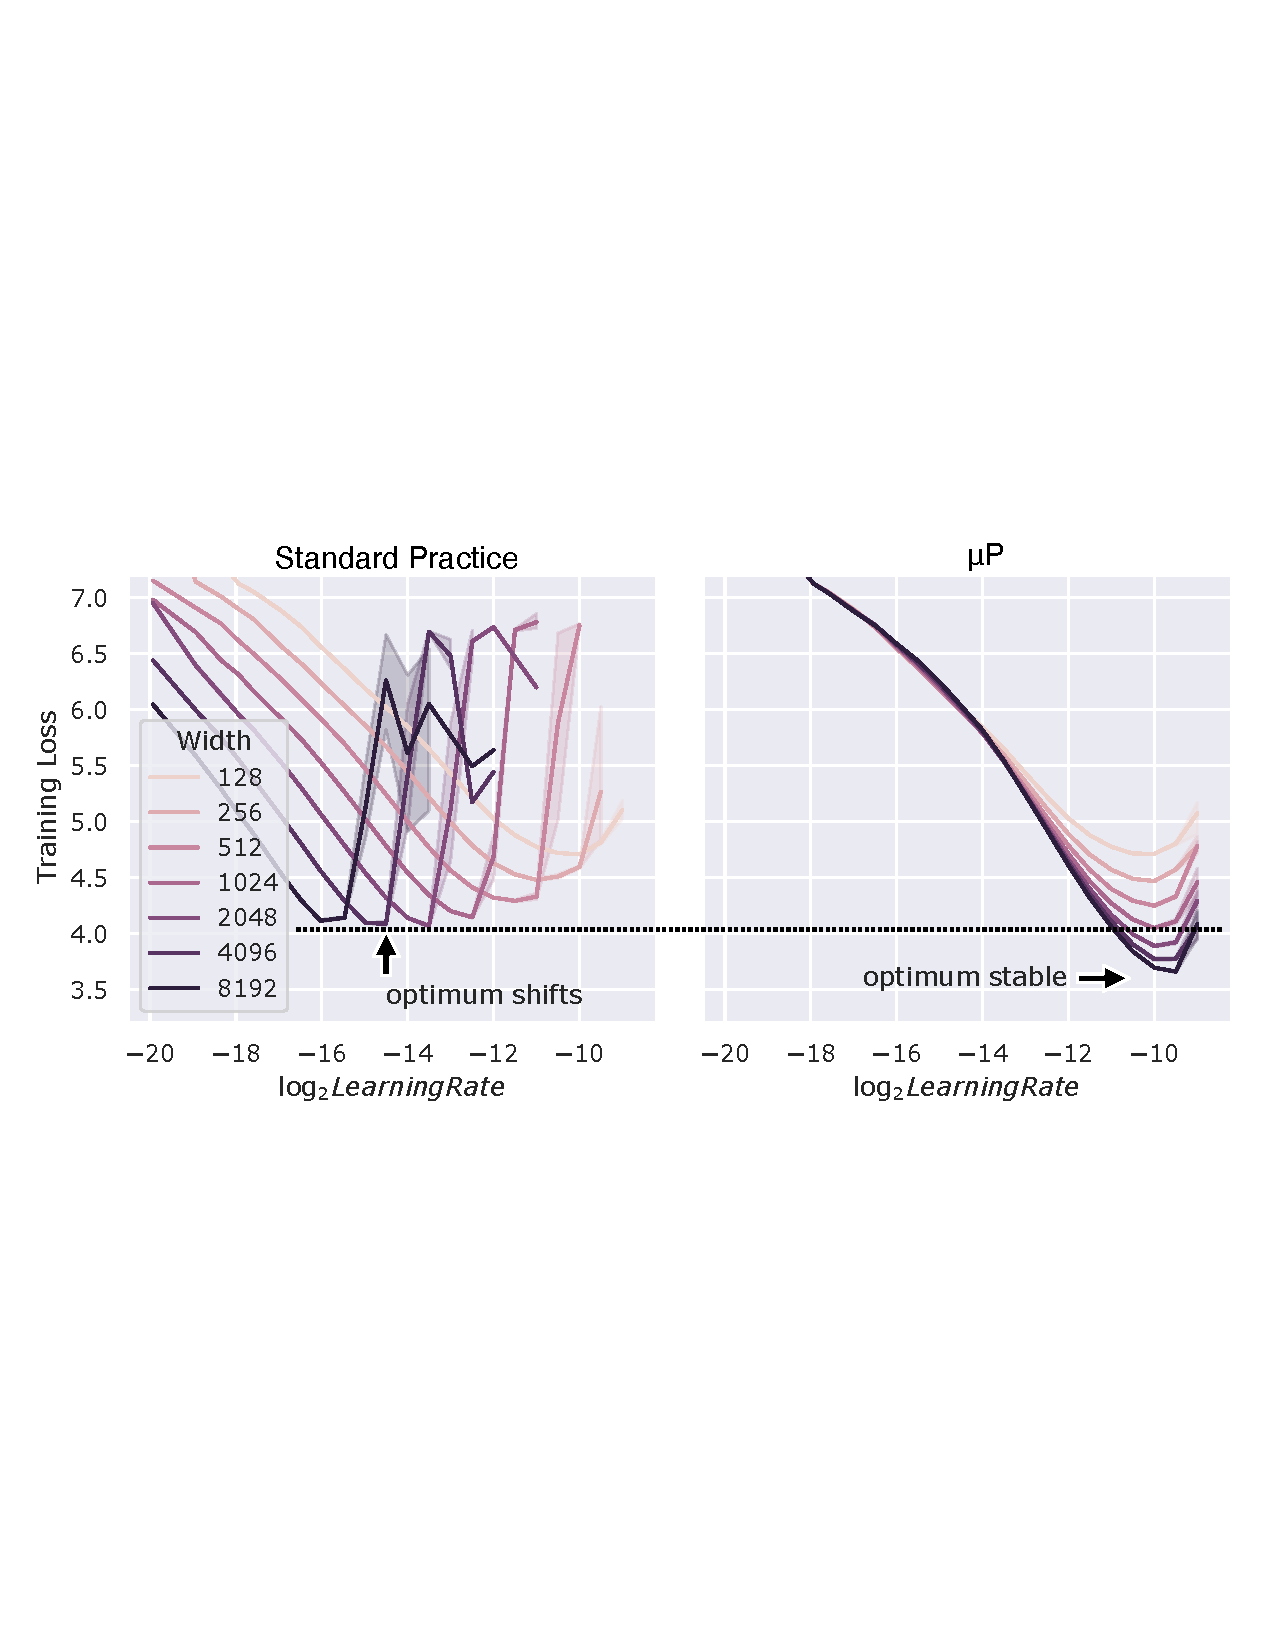
\includegraphics[width=14cm]{figs/hps/mup_img_flattened.pdf}
  \caption{
  \textbf{The theory of network parameterization permits learning rate transfer across widths.}
  Transformers of varying widths trained on WikiText-2 under standard parameterization (left) and $\mu$P (right).
  Under standard parameterization, the optimal learning rate decreases as model width increases.
  Under $\mu$P, by contrast, the optimal learning rate remains nearly constant across widths, making it possible to predict the learning rate for wide networks from experiments on narrower, cheaper models.
  Reproduced from \citet{yang2022tensor}.
  }
  \label{fig:hps-mup}
\end{figure}

\paragraph{Disentangling architecture hyperparameters from optimization hyperparameters.}
There has been a highly successful line of work aimed at disentangling \textit{architecture} hyperparameters such as width, depth, and output multiplier (see the lazy/rich dichotomy in \cref{sec:reason-limits}), from \textit{optimization} hyperparameters such as the learning rate and initialization variance.
The Tensor Programs framework \citep{yang2021tensor, yang2023tensor} makes this separation explicit, writing hyperparameters such as the learning rate in the form $\eta = \eta_0 \cdot [\mathrm{width}]^{c}$, separating a scale-independent coefficient $\eta_0$ from a width dependent factor with exponent $c$.
This line of work then asks: how can we set these exponents such that we retain interesting training behavior at infinite width?
A remarkable insight from this analysis is that all non-trivial and non-explosive scalings give one of two limiting behaviors, analogous to the rich/lazy dichotomy in \cref{sec:reason-limits}:
in the \textit{Neural Tangent Parameterization} (NTP), features are frozen during training, and in the \textit{Maximal Update Parameterization} ($\mu$P), features evolve.
Since feature learning is essential for most tasks, this analysis tells us that $\mu$P is the scaling to use, resolving how hyperparameters should scale with model width.
This understanding enables hyperparameter transfer: we can tune hyperparameters on small proxy models and then transfer them to large, production-size models, where they remain near-optimal when both models are sufficiently wide (\citep{yang2022tensor}; \cref{fig:hps-mup}).

At the same time, the theory underpinning this result is asymptotic and does not fully account for its empirical effectiveness.
In practice, models are trained at widths far smaller than the dataset size, and the usefulness of transfer depends on how \textit{quickly} optimal hyperparameters stabilize with width.
\citet{noci2024super} and \citet{ghosh2025understanding} and \citet{hayou2025proof} take steps toward closing this gap, providing evidence that a small set of spectral statistics stabilizes rapidly across widths under $\mu$P and approximately governs the optimal hyperparameters.
This scaling-centric approach to hyperparameters was later extended to depth scaling \citep{yang2023depth, bordelon2023depthwise, dey2025don}, and leveraging this approach with other scaling dimensions remains an important future direction (see \cref{openquestion:zero_hyperparameters}).
